\documentclass[11pt]{article}

\usepackage[a4paper,margin=2.4cm]{geometry}
\usepackage{amsmath,amssymb}
\usepackage{graphicx}
\usepackage{booktabs}
\usepackage{xcolor}
\usepackage{tikz}
\usetikzlibrary{arrows.meta,positioning,fit,backgrounds,calc}
\usepackage[font=small,labelfont=bf]{caption}
\usepackage{float}
\usepackage{enumitem}
\usepackage{microtype}
\usepackage[hidelinks]{hyperref}

\definecolor{lensorange}{HTML}{D98A00}
\definecolor{lensorangeb}{HTML}{F59E0B}
\definecolor{lensslate}{HTML}{3A3A42}
\definecolor{lensblue}{HTML}{4F7BF6}
\definecolor{lensgrey}{HTML}{6B6878}
\definecolor{lenspaper}{HTML}{F9F9FA}
\hypersetup{colorlinks=true,linkcolor=lensslate,urlcolor=lensblue}
\setlength{\parindent}{0pt}\setlength{\parskip}{0.55em}

\newcommand{\file}[1]{\texttt{\small #1}}
\newcommand{\code}[1]{\texttt{\small #1}}
\newcommand{\note}[2]{\begin{center}\small
  \fcolorbox{lensslate}{lenspaper}{\parbox{0.95\linewidth}{\textbf{\color{lensslate}#1.}\ #2}}\end{center}}

\title{\vspace{-1.4cm}
  
\includegraphics[height=1.25cm]{assets/lensing-logo.pdf}\\[0.7em]
  \textbf{Pathfinder, for Engineers}\\[0.2em]
  {\large How the Models and the Serverless Runtime Fit Together}}
\author{\textsc{lensing}\,\,$\cdot$\,\,spotify-pathfinder \quad\small(developer guide)}
\date{June 2026}

\begin{document}
\maketitle

\begin{abstract}\noindent
This is the engineer's tour of Pathfinder --- the app that draws a 3D ``musical journey'' between two
Spotify tracks. The interesting part is operational: it serves seven models from a \emph{single
Cloudflare Worker} with no Python origin and no vector DB at request time, by doing all the model
training offline and shipping the \emph{outputs} as a memory-mapped binary snapshot. The Rust/WASM
core then does only arithmetic (search, projection) under a ${\sim}10$\,ms CPU budget. We walk the
architecture, the request lifecycle, the snapshot format, each model at a practical level, and how to
rebuild it. Math is kept to what you need; file paths are given so you can read the source.
\end{abstract}

%====================================================================
\section{Architecture at a glance}

One Worker (\file{worker/index.ts}) serves the static UI \emph{and} answers \file{/api/*}. Everything
expensive was either precomputed offline or compiled to WASM (\file{worker-core/}). The split that
makes it fit:

\begin{itemize}[leftmargin=1.4em,itemsep=2pt]
\item \textbf{Offline build} (Python + Qdrant + torch): train the models, score the corpus, and write
three artifacts to \file{public/data/} --- \file{corpus.bin}, \file{transitions.json},
\file{projector.bin}.
\item \textbf{Request time} (Worker + WASM): on first hit per isolate, load the snapshot into the Rust
core; thereafter every route is graph search + linear algebra over \emph{frozen} model outputs. The
only model that runs live is the cold-start text embedding (Workers AI), and only for tracks not
already in the corpus.
\end{itemize}

\note{The constraint that shapes everything}{Workers Free gives ${\sim}10$\,ms CPU per request. You
cannot run gradient boosting or a torch encoder over 23k tracks in that budget --- but you \emph{can}
memory-map a precomputed table and do a bounded A\textsuperscript{*}. So the rule is: models produce
\textbf{data} offline; the Worker runs \textbf{algorithms} on that data.}

\begin{figure}[H]\centering
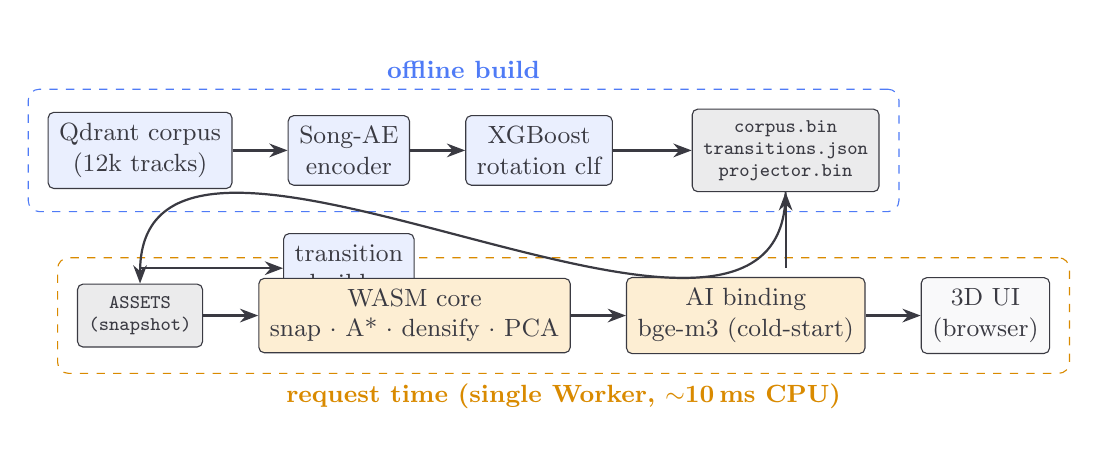
\begin{tikzpicture}[font=\small,
  box/.style={draw=lensslate,rounded corners=2pt,align=center,inner sep=4pt,minimum height=8mm},
  off/.style={box,fill=lensblue!12}, on/.style={box,fill=lensorangeb!18},
  art/.style={box,fill=lensslate!10,font=\ttfamily\scriptsize},
  ar/.style={-{Stealth[]},lensslate,thick}, every node/.style={text=lensslate}]
  \node[off] (qd) {Qdrant corpus\\(12k tracks)};
  \node[off,right=7mm of qd] (ae) {Song-AE\\encoder};
  \node[off,right=7mm of ae] (xgb) {XGBoost\\rotation clf};
  \node[off,below=6mm of ae] (tr) {transition\\builder};
  \node[art,right=10mm of xgb] (snap) {corpus.bin\\transitions.json\\projector.bin};
  \draw[ar] (qd)--(ae); \draw[ar] (ae)--(xgb); \draw[ar] (qd|-tr)--(tr);
  \draw[ar] (xgb)--(snap); \draw[ar] (tr-|snap)--(snap);
  \node[art,below=12mm of qd] (asset) {ASSETS\\(snapshot)};
  \node[on,right=7mm of asset] (wasm) {WASM core\\snap $\cdot$ A* $\cdot$ densify $\cdot$ PCA};
  \node[on,right=7mm of wasm] (ai) {AI binding\\bge-m3 (cold-start)};
  \node[box,fill=lenspaper,right=7mm of ai] (ui) {3D UI\\(browser)};
  \draw[ar] (asset)--(wasm); \draw[ar] (wasm)--(ai); \draw[ar] (ai)--(ui);
  \draw[ar] (snap) to[out=-90,in=90] (asset);
  \begin{scope}[on background layer]
    \node[draw=lensblue,dashed,rounded corners,fit=(qd)(snap),inner sep=7pt,label={[lensblue]above:\textbf{offline build}}]{};
    \node[draw=lensorange,dashed,rounded corners,fit=(asset)(ui),inner sep=7pt,label={[lensorange]below:\textbf{request time (single Worker, ${\sim}$10\,ms CPU)}}]{};
  \end{scope}
\end{tikzpicture}
\caption{Train offline (blue), infer at the edge (orange). The Worker reads frozen outputs.}
\end{figure}

%====================================================================
\section{The request lifecycle}

A \file{POST /api/route} with \code{\{start\_uri, end\_uri, length, context\}} flows like this
(\file{worker/index.ts} $\rightarrow$ \file{worker-core/src/lib.rs}):

\begin{enumerate}[leftmargin=1.5em,itemsep=2pt]
\item \textbf{ensureReady} (once per isolate): \code{initSync} the WASM module, fetch the three
snapshot files via the \code{ASSETS} binding, \code{load\_corpus} + \code{set\_projector}.
\item \textbf{resolveEndpoint} for each track: \code{find\_row(uri)}. If in corpus $\rightarrow$ use
its baked vector. If not $\rightarrow$ \emph{cold-start}: fetch Spotify/ReccoBeats metadata, embed via
the AI binding, \code{project\_and\_snap} to the nearest corpus anchor.
\item \textbf{wasmRoute(startRow, endRow, \dots)}: A\textsuperscript{*} over the $k$-NN graph,
\code{densify} to the requested length, gather a neighbor ``cloud'', run PCA to 3-d, return JSON
(nodes with positions + per-hop ``why'').
\item The Worker adds snap edges for any cold-start endpoints and returns the route.
\end{enumerate}

Other endpoints: \file{/api/search} (Spotify search, cached; falls back to corpus search),
\file{/api/preview} (30\,s clips via Deezer$\rightarrow$iTunes), \file{/api/config} (public Spotify
client id for the browser PKCE playlist flow).

%====================================================================
\section{The snapshot (what the Worker actually reads)}

\file{corpus.bin} (\code{PFC1}) is the whole map in one memory-mapped blob: $n{=}23{,}529$ tracks,
64-d L2-normalized vectors, a per-track \code{fit} score, the $k{=}20$ neighbor graph (indices +
cosine distances), and a small JSON meta block (uri/name/artist/album/genre). \file{transitions.json}
holds the bigram/back-off/context tables. \file{projector.bin} (\code{PFP1}) holds the cold-start
MLP weights + its feature config. Layouts:

\begin{table}[H]\centering\small
\begin{tabular}{@{}llll@{}}
\toprule
\multicolumn{2}{c}{\code{PFC1} corpus.bin} & \multicolumn{2}{c}{\code{PFP1} projector.bin}\\
\cmidrule(r){1-2}\cmidrule(l){3-4}
field & type & field & type \\
\midrule
magic\,/\,ver\,/\,$n$\,/\,dim\,/\,$k$ & \code{u32}$\times$5 & magic\,$\dots$\,in\,/\,$h$\,/\,out\,/\,text & \code{u32}$\times$6 \\
ids & \code{u64}$[n]$ & $W_1, b_1$ & \code{f32} \\
vecs (L2-norm) & \code{f32}$[n{\cdot}64]$ & $W_2, b_2$ & \code{f32} \\
fit & \code{f32}$[n]$ & cfg\_len & \code{u32} \\
nbr\_idx / nbr\_dist & \code{u32/f32}$[n{\cdot}k]$ & cfg (stats, vocab) & JSON \\
meta\_len {+} JSON & \code{u32}{+}bytes & & \\
\bottomrule
\end{tabular}
\caption{Little-endian; parsed in \file{snapshot.rs} / \file{project.rs}. Distances are baked, so a
graph move at request time is a table lookup, not a dot product.}
\end{table}

%====================================================================
\section{The models, practically}

\subsection{The map --- Song autoencoder}
An MLP autoencoder ($539\to256\to64$, trained offline) embeds each track into a 64-d space where
cosine distance means ``musically similar''. You never run it in the Worker; you consume its output
(the \code{vecs} in \file{corpus.bin}). This space is the coordinate system for the $k$-NN graph, the
A\textsuperscript{*} heuristic, and the 3D view. Its 539-d input stitches together a text embedding,
numeric stats, acoustic features (+ missing flags), and genre/album one-hots (Figure~\ref{fig:blocks},
left).

\begin{figure}[H]\centering
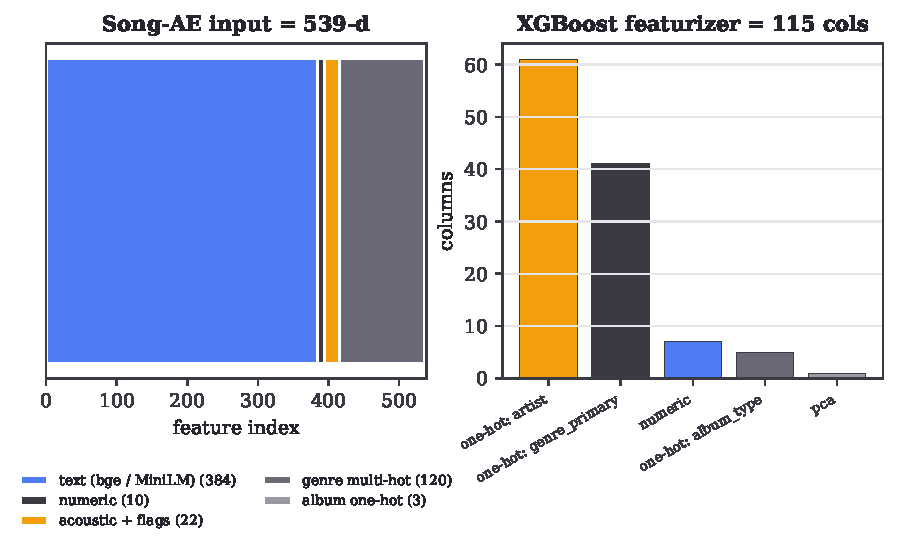
\includegraphics[width=\linewidth]{figures/fig_feature_blocks.pdf}
\caption{Left: the 539-d Song-AE input by modality. Right: the \emph{separate} 115-column featurizer
the \code{fit} classifier uses --- mostly identity one-hots, not dense vectors.}
\label{fig:blocks}
\end{figure}

\subsection{The \code{fit} score --- XGBoost rotation classifier}
\code{fit} is the per-track number A\textsuperscript{*} uses to prefer ``sticky'' tracks. It is the
probability of \textbf{rotation} --- \code{play\_count >= 2}, ``did the listener come back?'' --- from
an XGBoost binary classifier (\code{binary:logistic}), scored over the corpus offline, min--max
normalized, and stored as the \code{fit} column. Test \textbf{AUC 0.7429}.

\note{The lesson worth internalizing}{The classifier's features are \emph{identity} one-hots (artist,
genre) in trees, not dense embeddings. The project tried the obvious dense features --- a content-text
embedding, audio features, even the Song-AE latent --- and they all \emph{hurt or diluted} the score
(Figure~\ref{fig:bakeoff}). So the Song-AE latent is great as map \emph{geometry} but a poor
\emph{feature} for the fit model; they are deliberately separate featurizers. Corollary: scan
dataset/feature choices before you tune trees.}

\begin{figure}[H]\centering
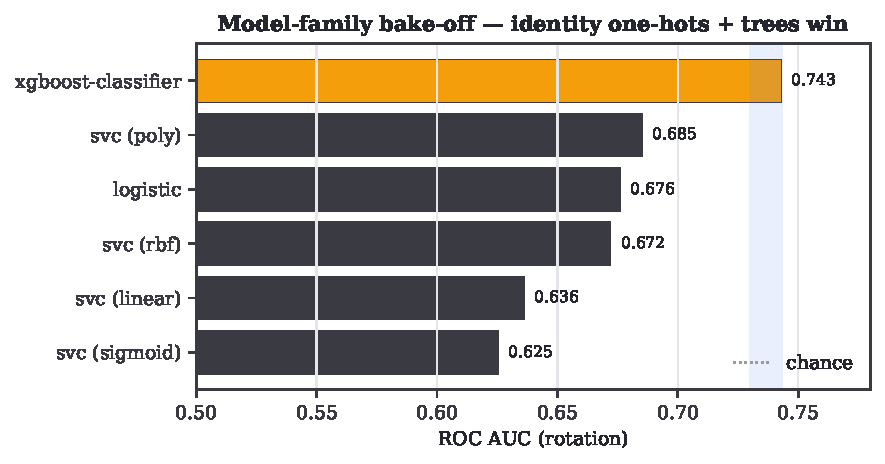
\includegraphics[width=0.78\linewidth]{figures/fig_bakeoff.pdf}
\caption{Real logged runs: the tree on identity one-hots beats every dense distance/margin model
(SVC kernels, logistic) by several noise bands. Dense embeddings did not help the \code{fit} target.}
\label{fig:bakeoff}
\end{figure}

\subsection{Cold-start --- the distilled projector}
For off-map tracks you must produce a 64-d vector \emph{in the Worker}. You can't run the real torch
encoder there, so the build trains a small ``projector'' MLP ($1179\to256\to64$) to \emph{reproduce}
the Song-AE latents from features you can fetch live (a \code{bge-m3} text embedding via the AI
binding + numeric/acoustic/genre/album blocks). It is a lossy translator, so the result is immediately
snapped to the nearest real corpus anchor.

\textbf{One detail worth copying:} acoustic features from ReccoBeats are often missing. Because inputs
are z-scored, an imputed mean lands at \emph{exactly $0$} --- indistinguishable from a genuinely
average track. So each acoustic feature ships \emph{two} inputs: the value and a 0/1 ``was-this-real''
flag. Mean-imputation made honest.

\subsection{The transition model --- bigram with back-off}
A\textsuperscript{*} also prefers transitions real sessions make. From a sessionized play log, the
build forms a satisfaction-weighted track bigram, backing off to artist/genre when a track is rarely
observed: it trusts the bigram in proportion to its support $n_u$ (the count of recorded successors),
$\tau=n_u/(n_u+8)$ --- think ``real observations / (real + 8 prior) observations''. Time-of-day and
shuffle add multiplicative \emph{lifts} (how over/under-represented a genre is in a context).
Figure~\ref{fig:lifts} shows the real patterns --- and that the daily rhythm is a genre phenomenon,
not a release-era one.

\begin{figure}[H]\centering
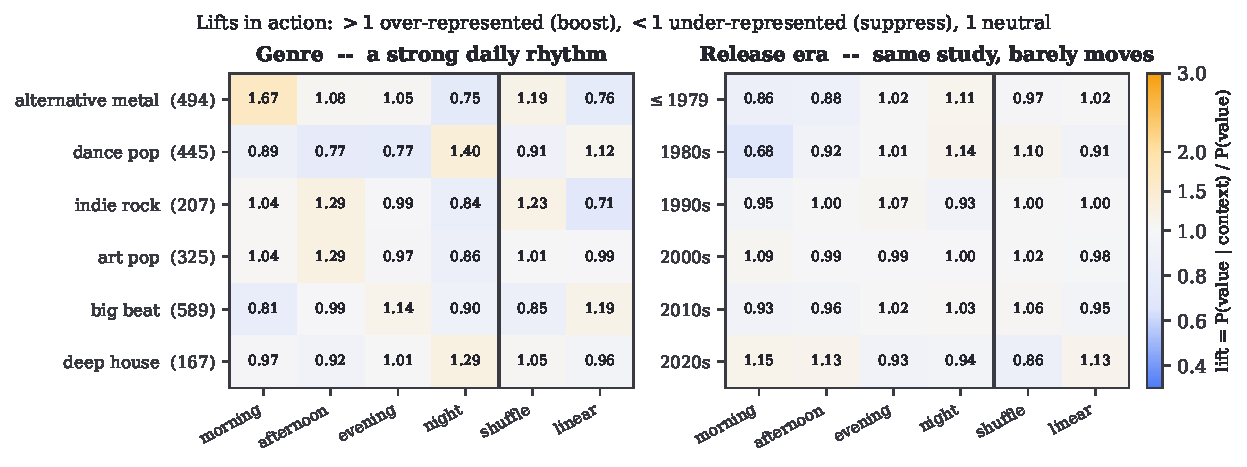
\includegraphics[width=\linewidth]{figures/fig_lifts.pdf}
\caption{Real genre lifts (left) vs.\ the same study on release era (right). $>1$ boost, $<1$
suppress. Genre swings hard with time-of-day and shuffle; era barely moves.}
\label{fig:lifts}
\end{figure}

\subsection{Pathfinding --- A\textsuperscript{*} + densify}
A\textsuperscript{*} on the $k$-NN graph, heuristic = cosine distance to the goal. Each hop's cost is
a weighted sum of five interpretable terms (no magic):
\begin{center}\small
\begin{tabular}{@{}lll@{}}
\toprule
term & weight & meaning \\
\midrule
distance & 1.0 & cosine step on the map \\
fit & 0.5 & prefer high-\code{fit} (sticky) tracks \\
diversity & 0.5 & small penalty ($\gamma{=}0.15$) for a genre change \\
transition & 0.6 & prefer learned next-track affinity \\
context & 0.4 & prefer time-of-day / shuffle fit \\
\bottomrule
\end{tabular}
\end{center}
Hard constraints: no repeats, $\le 2$ same-artist in a row, no artist over $\lceil L/4\rceil$ of an
$L$-track route. \code{densify} fills short routes by inserting the best track into the widest gap.
The search is capped at \code{MAX\_EXPANSIONS = 45{,}000} and returns a clean 404 instead of blowing
the CPU slice (a 503). The weights are constants; Figure~\ref{fig:astar} shows how the found path
responds to them.

\begin{figure}[H]\centering
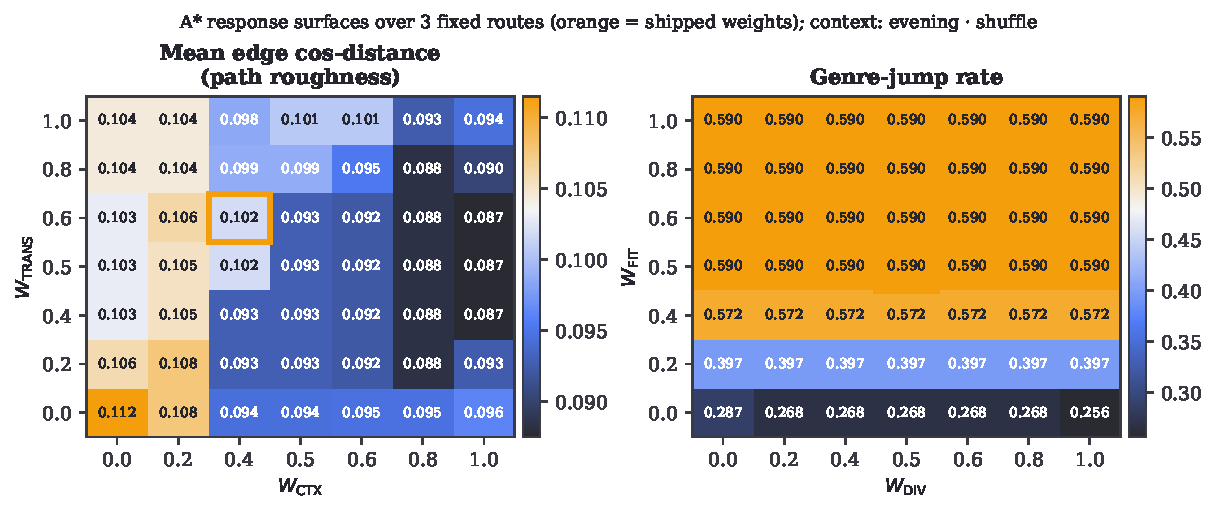
\includegraphics[width=\linewidth]{figures/fig_astar_sweep.pdf}
\caption{A\textsuperscript{*} weight response surfaces over the real corpus (orange = shipped). More
context weight $\Rightarrow$ smoother paths; the genre-diversity penalty is gentle.}
\label{fig:astar}
\end{figure}

\subsection{$k$-NN graph and PCA}
The graph is symmetric $k{=}20$ cosine neighbors, baked into \file{corpus.bin} (so graph moves are
lookups). The 3D view projects the path+cloud from 64-d via power-iteration PCA per request --- cheap
because the covariance is only $64\times64$ over ${\sim}100$ points, and it avoids an SVD dependency
in WASM.

%====================================================================
\section{Worked example: one route, end to end}

To make the chain concrete, here is a single real request traced through every stage, with the actual
numbers (regenerate with \file{docs/sweeps/run\_example.py}). The ask: route from \emph{Kraftwerk --
``Tour de France''} to \emph{Muse -- ``Intro''}, context \emph{evening$\cdot$shuffle}. Both are in the
corpus, so no cold-start; the search runs on the baked graph.

\begin{figure}[H]\centering
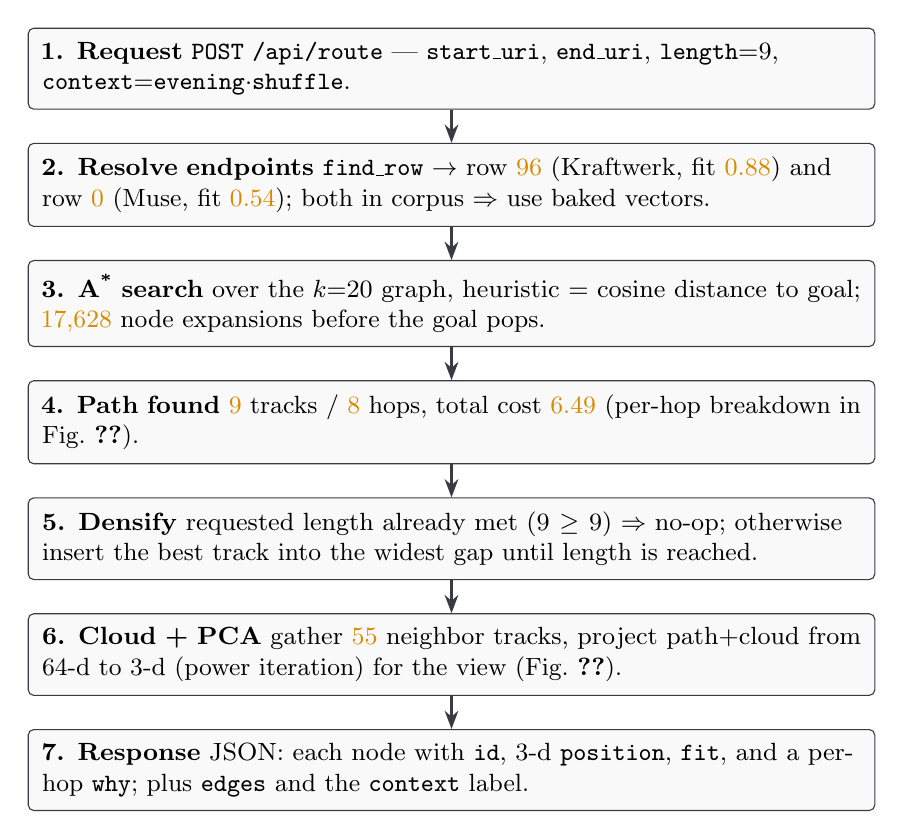
\begin{tikzpicture}[font=\small,node distance=4.2mm,
  st/.style={draw=lensslate,rounded corners=2pt,align=left,inner sep=5pt,text width=10.4cm,fill=lenspaper},
  num/.style={lensorange},
  ar/.style={-{Stealth[]},lensslate,thick}]
  \node[st] (s1) {\textbf{1. Request} \file{POST /api/route} --- \code{start\_uri}, \code{end\_uri},
    \code{length}=9, \code{context}=\code{evening$\cdot$shuffle}.};
  \node[st,below=of s1] (s2) {\textbf{2. Resolve endpoints} \code{find\_row} $\to$ row {\color{lensorange}96}
    (Kraftwerk, fit {\color{lensorange}0.88}) and row {\color{lensorange}0} (Muse, fit
    {\color{lensorange}0.54}); both in corpus $\Rightarrow$ use baked vectors.};
  \node[st,below=of s2] (s3) {\textbf{3. A\textsuperscript{*} search} over the $k{=}20$ graph,
    heuristic $=$ cosine distance to goal; {\color{lensorange}17{,}628} node expansions before the goal
    pops.};
  \node[st,below=of s3] (s4) {\textbf{4. Path found} {\color{lensorange}9} tracks /
    {\color{lensorange}8} hops, total cost {\color{lensorange}6.49} (per-hop breakdown in
    Fig.~\ref{fig:excost}).};
  \node[st,below=of s4] (s5) {\textbf{5. Densify} requested length already met ($9\ge9$) $\Rightarrow$
    no-op; otherwise insert the best track into the widest gap until length is reached.};
  \node[st,below=of s5] (s6) {\textbf{6. Cloud + PCA} gather {\color{lensorange}55} neighbor tracks,
    project path$+$cloud from 64-d to 3-d (power iteration) for the view (Fig.~\ref{fig:expath}).};
  \node[st,below=of s6] (s7) {\textbf{7. Response} JSON: each node with \code{id}, 3-d
    \code{position}, \code{fit}, and a per-hop \code{why}; plus \code{edges} and the \code{context}
    label.};
  \foreach \a/\b in {s1/s2,s2/s3,s3/s4,s4/s5,s5/s6,s6/s7} \draw[ar] (\a)--(\b);
\end{tikzpicture}
\caption{The full request chain for the example route, with real numbers at each stage.}
\label{fig:chain}
\end{figure}

\textbf{The journey it returns.} The nine tracks weave across genres while the straight-line distance
to the Muse endpoint ($h$) falls steadily --- that shrinking $h$ is the heuristic pulling the search
home (Figure~\ref{fig:strip}).

\begin{figure}[H]\centering
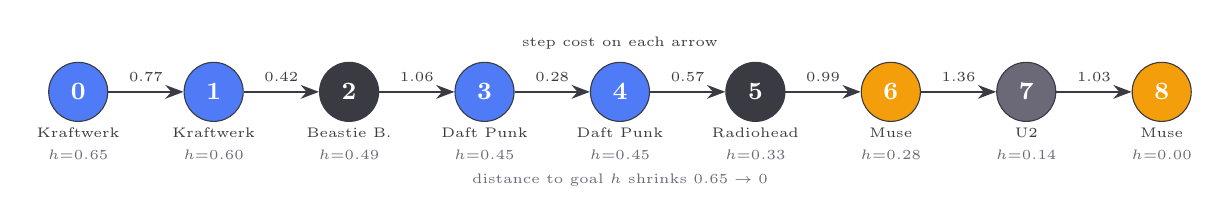
\begin{tikzpicture}[x=1.72cm,y=1cm,font=\small,
  gnode/.style={circle,draw=lensslate,text=white,minimum size=7.5mm,inner sep=0,font=\small\bfseries}]
  \foreach [count=\i from 0] \num/\art/\col/\hh in {%
    0/Kraftwerk/lensblue/0.65, 1/Kraftwerk/lensblue/0.60, 2/{Beastie B.}/lensslate/0.49,
    3/{Daft Punk}/lensblue/0.45, 4/{Daft Punk}/lensblue/0.45, 5/Radiohead/lensslate/0.33,
    6/Muse/lensorangeb/0.28, 7/U2/lensgrey/0.14, 8/Muse/lensorangeb/0.00}{
      \node[gnode,fill=\col] (n\num) at (\i,0) {\num};
      \node[font=\tiny,text=lensslate] at (\i,-0.52) {\art};
      \node[font=\tiny,text=lensgrey] at (\i,-0.80) {$h{=}\hh$};
  }
  \foreach \a/\b/\s in {0/1/0.77,1/2/0.42,2/3/1.06,3/4/0.28,4/5/0.57,5/6/0.99,6/7/1.36,7/8/1.03}{
      \draw[-{Stealth[]},lensslate,thick] (n\a)--(n\b) node[midway,above,font=\tiny,text=lensslate]{\s};
  }
  \node[font=\tiny,text=lensslate] at (4,0.62) {step cost on each arrow};
  \node[font=\tiny,text=lensgrey] at (4,-1.12) {distance to goal $h$ shrinks $0.65 \to 0$};
\end{tikzpicture}
\caption{The route as a journey. Node colour $=$ genre family: blue $=$ electronic (Düsseldorf /
electro), slate $=$ alternative rock, orange $=$ modern rock, grey $=$ irish rock. Numbers on arrows
are the per-hop A\textsuperscript{*} cost; $h$ under each node is the cosine distance still to go.}
\label{fig:strip}
\end{figure}

The full step-by-step (genre arc: electronic $\to$ alt-rock $\to$ electro $\to$ alt-rock $\to$ rock):

\begin{table}[H]\centering\small
\begin{tabular}{@{}rlllrr@{}}
\toprule
\# & track / artist & genre & \code{fit} & step cost & dominant term \\
\midrule
0 & Tour de France --- Kraftwerk & dusseldorf electronic & 0.88 & --- & (start) \\
1 & (Kraftwerk) & dusseldorf electronic & 0.84 & 0.77 & transition \\
2 & (Beastie Boys) & alternative rock & 0.58 & 0.42 & fit \\
3 & (Daft Punk) & electro & 0.68 & 1.06 & transition \\
4 & (Daft Punk) & electro & 0.87 & 0.28 & distance \\
5 & (Radiohead) & alternative rock & 0.87 & 0.57 & context \\
6 & (Muse) & modern rock & 0.50 & 0.99 & transition \\
7 & (U2) & irish rock & 0.19 & 1.36 & fit + transition \\
8 & Intro --- Muse & modern rock & 0.54 & 1.03 & transition \\
\bottomrule
\end{tabular}
\caption{The 9-track route. ``Dominant term'' is the largest contributor to that hop's cost. The
priciest hop (7, $\to$ U2) is driven by U2's low \code{fit} $0.19$: the fit term alone is
$0.5(1-0.19)=0.40$.}
\end{table}

\subsection*{The decision at each step}

At every track A\textsuperscript{*} sees up to 20 graph neighbors (minus any blocked by the no-repeat
and artist-cap constraints) and must choose one to extend toward. The key thing to understand is that
it does \emph{not} pick the locally-cheapest next step: it commits to the neighbor that lies on the
cheapest \emph{complete} route to the goal. Figure~\ref{fig:decisions} shows this directly --- the
orange ``chosen'' step often sits \emph{above} cheaper options it passed over (blue rings).

\begin{figure}[H]\centering
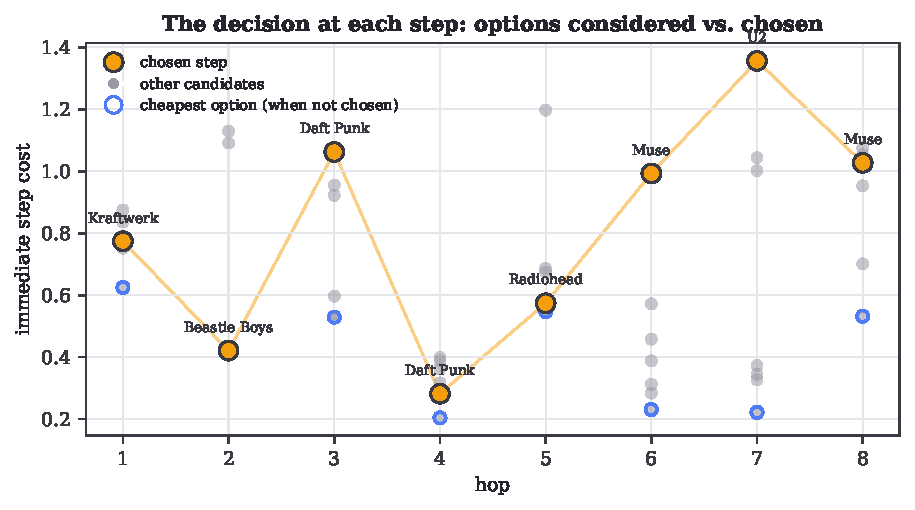
\includegraphics[width=0.92\linewidth]{figures/fig_example_decisions.pdf}
\caption{Every hop's menu. Grey dots are the candidate next-tracks A\textsuperscript{*} weighed
(by immediate step cost); orange is the one it committed to; a blue ring marks the cheapest option
when that was \emph{not} chosen. At hops 6 and 7 it deliberately pays ${\sim}1.0$--$1.4$ to leave a
cluster, skipping ${\sim}0.2$ stay-put steps --- because those cheap steps don't actually reach Muse.}
\label{fig:decisions}
\end{figure}

Walking the decisions (Figure~\ref{fig:strip} for the path, \ref{fig:excost} for the cost split):
\begin{itemize}[leftmargin=1.4em,itemsep=2pt]
\item \textbf{Hop 2 --- the bridge out (Kraftwerk\,$\to$\,Beastie Boys).} The cheapest available step
\emph{and} a genre jump that drops $h$ from $0.60$ to $0.49$. Easy call: leave electronic for the
rock side of the map exactly when it also makes progress.
\item \textbf{Hop 3 --- a costly detour (\,$\to$\,Daft Punk, electro).} Locally a Blur step looked
cheaper ($0.53$ vs $1.06$), but A\textsuperscript{*} took the pricier electro hop because it sets up a
cheaper remainder --- greedy would have missed it.
\item \textbf{Hop 4 --- the easy glide (Daft Punk\,$\to$\,Daft Punk).} Short on the map and high-fit
($0.87$): the cheapest hop in the route at $0.28$, an in-cluster step.
\item \textbf{Hops 6--7 --- leaving the cluster (\,$\to$\,Muse,\,$\to$\,U2).} Six cheaper Radiohead/Muse
steps (${\sim}0.2$) were on offer, but the consecutive-artist cap (max 2) and the goal pull make the
jumps worth it; U2 costs the most ($1.36$, its \code{fit} is only $0.19$) yet it is the bridge that
brings $h$ down to $0.14$, one short hop from the Muse endpoint.
\end{itemize}

\begin{figure}[H]\centering
\begin{minipage}[t]{0.52\linewidth}\centering
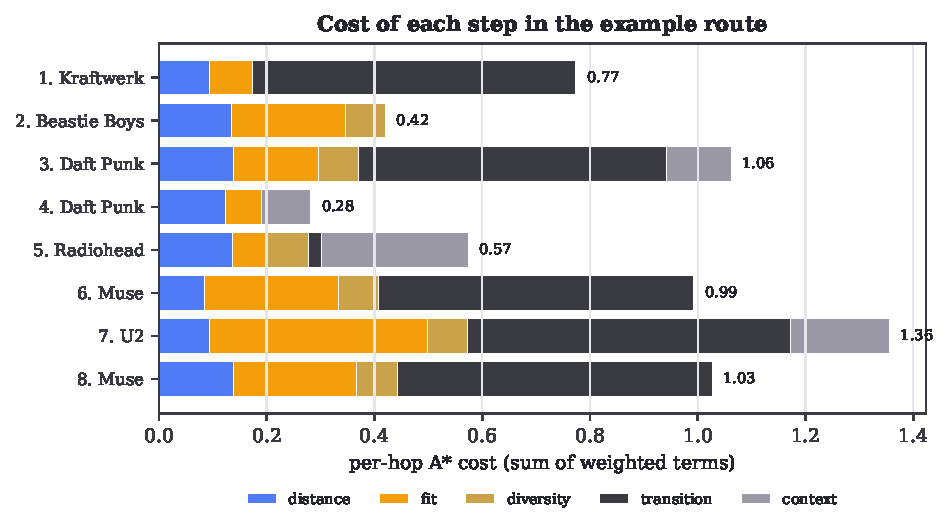
\includegraphics[width=\linewidth]{figures/fig_example_cost.pdf}
\end{minipage}\hfill
\begin{minipage}[t]{0.46\linewidth}\centering
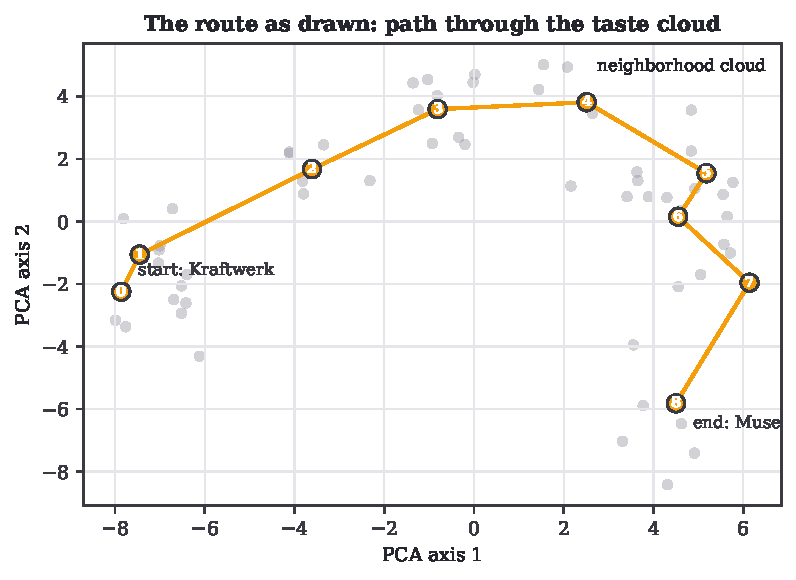
\includegraphics[width=\linewidth]{figures/fig_example_path.pdf}
\end{minipage}
\caption{\textbf{Left} (\ref{fig:excost}): each chosen hop's cost split into the five weighted terms
--- \emph{why} that step cost what it did. \textbf{Right} (\ref{fig:expath}): the same route as the UI
draws it, threading through the grey neighborhood cloud in the PCA plane.}
\label{fig:excost}\label{fig:expath}
\end{figure}

%====================================================================
\section{Validation}
The request-time core is a Rust rewrite of Python references, so a \textbf{parity test}
(\file{worker-core/tests/parity.rs}) checks A\textsuperscript{*} against \file{search.py}: same
endpoints/length, constraints satisfied, Rust cost $\le 1.6\times$ Python $+\,0.1$, $\ge 85\%$ node
identity. (Heuristic search legitimately produces alternate near-optimal paths, so exact match is the
wrong bar.) A round-trip test guards the projector binary. Model deltas are judged against a measured
noise band $\sigma_{\text{AUC}}=0.0063$ --- e.g.\ a freshly-run depth/lr scan finds a best AUC of
0.7534, only $+0.011$ over the shipped config, i.e.\ inside $2\sigma$ (Figure~\ref{fig:xgb}).

\begin{figure}[H]\centering
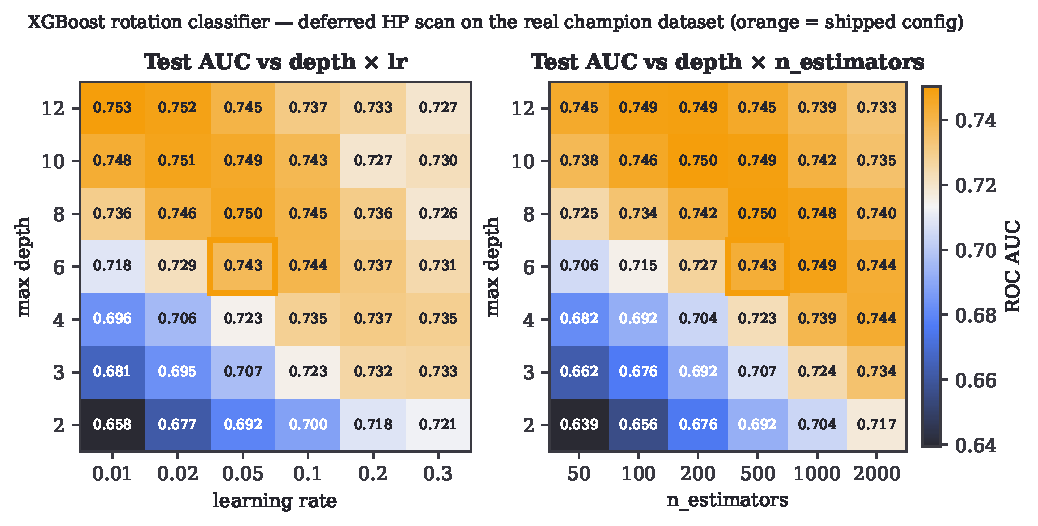
\includegraphics[width=\linewidth]{figures/fig_xgb_sweep.pdf}
\caption{The deferred hyperparameter scan, run on the real dataset for this guide. Tuning moves AUC
less than seed noise --- don't over-invest in it.}
\label{fig:xgb}
\end{figure}

%====================================================================
\section{Build \& reproduce}
\begin{quote}\small\ttfamily
npm run build:snapshot\ \ \# Qdrant -> public/data/* (add --projector for cold-start)\\
npm run build\ \ \ \ \ \ \ \ \ \# wasm-pack -> tsc -> vite (copies data into dist)\\
npm run cf:dev\ \ \ \ \ \ \ \ \# wrangler dev at 127.0.0.1:8787
\end{quote}
Figures/sweeps in this guide regenerate via \file{docs/sweeps/*.py} + \file{docs/make\_figures.py};
the analysis dataset and logged runs live in the sibling \file{spotify-predict-engagement}. For the
full math (loss functions, the projector forward pass, PCA derivation, exact constants), see the
companion \emph{Models of Pathfinder} paper.

\end{document}
